\documentclass[12pt, a4paper]{report}
\usepackage{graphicx}
\usepackage{amsmath}

\graphicspath{{.}}

\title{First documuent}
\author{Peacesong \thanks{motivated by 2020-1 DL class}}
\date{\today}



\begin{document}

\maketitle

Title has been added to \LaTeX{} document!
% This line here is a comment. It will not be printed in the document.

This word will be in \textbf{bold,}
and this one in \underline{underline,}
finally this one in \textbf{\underline{\textit{bold, underline, and italic.}}}

The universe is immense and it seems to be homogeneous, in a large scale, everywhere we look at.

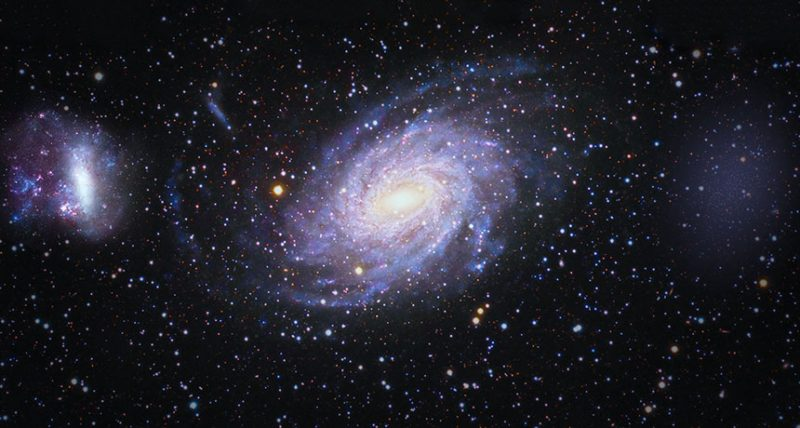
\includegraphics[width=0.25\textwidth]{galaxy}

Above is a picture of our galaxy, the Milky Way.

\begin{figure}[h]
  \centering
  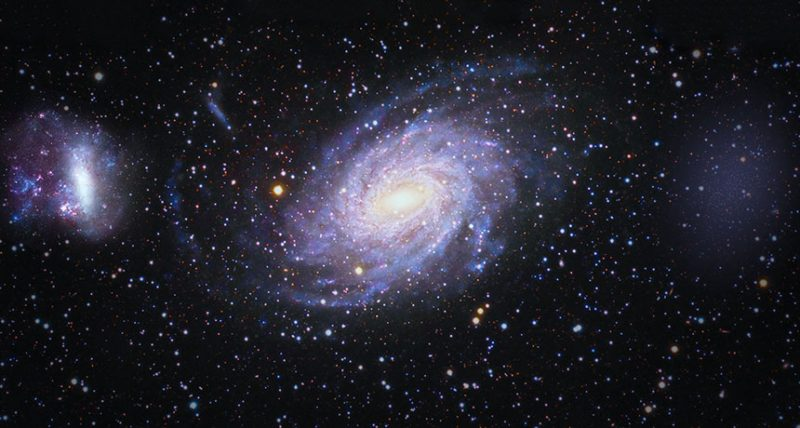
\includegraphics[width=0.25\textwidth]{galaxy}
  \caption{supposed to be a caption}
  \label{fig:mesh1}
\end{figure}

Above is an example of LaTeX caption of the figure \ref{fig:mesh1}. This is the reference to the page of it, the page \pageref{fig:mesh1}.

\begin{itemize}
  \item The individual entries are indicated with a black dot, a so-called bullet.
  \item The text in the entries may be of any length.
\end{itemize}

\begin{enumerate}
  \item Republic of Korea is an democratic republic.
  \item All power derive from the people.
\end{enumerate}

In phycis, the mass-energy equivalence is stated by the equation $E=mc^2$, discovered in 1905 by Alert Einstein.

The mass-energy equivalence is described by the famous equation \[E=mc^2 \] discovered in 1905 by Albert Einstein.
In natural units ($c = 1$), the formula expresses the identity
\begin{equation}
E=m
\end{equation}

Superscript: $e^{ix}$

Subscript: $p_i$

\[T^{i_1 i_2 \dots i_p}_{j_1 j_2 \dots j_p} = T(x^{i_1}, x^{i_2}, \dots, x^{i_p}, e_{j_1}, e_{j_2}, \dots, e_{j_p}) \]

\begin{equation*}
\int_0^1 \frac{1}{x} dx \\
\omega^2 + \omega + 1 = 0 \\
\delta \Delta \\
O(n) \Omega(n) o(n) \\
\sin(\alpha+\beta) = \sin(\alpha)\cos(\beta) + \sin(\beta)\cos(\alpha)
\end{equation*}

Whan that Aprille, with his shoures soote,\newline
The droughte of Marche, hath perced to the roote,

\chapter{First Chapter}

\section{Introduction}

Lorem ipsum dolor sit amet, consectetur adipiscing elit. Nunc sit amet odio facilisis, placerat risus quis, commodo ipsum. Sed dolor urna, accumsan in augue vel, viverra blandit diam. Aliquam urna magna, vestibulum a magna at, malesuada porttitor mi. Mauris non tincidunt dui. Vivamus sed sem eu massa efficitur euismod. Pellentesque feugiat mattis tortor eu egestas. Suspendisse eleifend nisl eu tortor congue, id bibendum risus vestibulum. Integer id sollicitudin mauris. Nam ut est ut sem facilisis viverra ut eu nulla.

\section{First Section}

Curabitur hendrerit sem et sapien porta, sed scelerisque ante vehicula. Integer vitae felis ut velit porta semper. Duis interdum odio nec lectus porttitor, ut sollicitudin lorem cursus. In faucibus turpis nec sollicitudin lobortis. Ut facilisis ipsum ac lorem aliquet, vel dapibus sapien gravida. In mattis mauris augue. Curabitur accumsan feugiat lectus, ac tempus augue posuere sit amet. Vivamus imperdiet pellentesque nibh, malesuada volutpat mauris porttitor vitae. Proin a cursus felis. Donec hendrerit molestie felis, vitae venenatis quam congue at. Nullam pulvinar ultrices metus, at posuere quam placerat eget. Praesent non dolor ipsum. Morbi sit amet sem rutrum, sollicitudin erat vitae, imperdiet est. Aenean ullamcorper dictum massa vitae pulvinar. Interdum et malesuada fames ac ante ipsum primis in faucibus. Praesent malesuada lectus eget quam molestie vestibulum.

\section{Second Section}

Quisque erat felis, rhoncus quis ultricies sit amet, consequat vitae odio. Fusce id commodo dolor. Quisque sed odio eu nisl efficitur lacinia in sed nunc. Maecenas congue in risus non mollis. Aenean erat libero, aliquet in placerat quis, feugiat quis nunc. Vestibulum at ante et ipsum tempus tempor. Sed vel blandit mi, a fermentum erat.

\subsection{A note to the readers}

Etiam interdum elit nec magna pretium, at ultrices neque fringilla. Vestibulum placerat magna vel venenatis feugiat. In consequat mattis felis in sodales. Ut sit amet tortor et diam molestie laoreet. Vestibulum nec luctus ex. Etiam in mi convallis, auctor ante sit amet, mattis ex. Nulla leo leo, aliquam ut scelerisque interdum, malesuada id mauris. Phasellus in lorem arcu. Lorem ipsum dolor sit amet, consectetur adipiscing elit. Maecenas ultrices at turpis in pellentesque. Donec lobortis sodales erat non varius. Phasellus felis ante, feugiat a tortor at, pulvinar semper lacus. Integer condimentum lobortis lectus a pretium. Proin cursus ultrices aliquam. Morbi suscipit nibh vitae ligula rutrum, sed imperdiet tortor tristique.


\begin{table}[h!]
\centering
\begin{tabular}{c c c}
  $a_{11}$ & $a_{12}$ & $a_{13}$ \\
  $a_{21}$ & $a_{22}$ & $a_{23}$ \\
  $a_{31}$ & $a_{32}$ & $a_{33}$ 
\end{tabular}
\caption{An example of 3x3 matrix from \LaTeX{}.}
\label{table:data}
\end{table}

Table \ref{table:data} is an example of a 3x3 matrix.

\begin{center}
\begin{tabular}{|c|c|c|}
  \hline
  1 & 0 & 0 \\
  \hline
  0 & 1 & 0 \\
  \hline
  0 & 0 & 1 \\
  \hline 
\end{tabular}
\end{center}



\end{document}
